\documentclass[8pt]{beamer}
\usepackage{amsmath}
\usepackage{amssymb}
\usepackage{graphicx}
\usepackage{hyperref}
\usepackage{color}
\usepackage{float}
\usepackage{subfig}


%\usepackage{sidecap}
\title{Random loops model can explain the appearance of Topologically Associating Domains (TADs)}
\author{Ofir Shukron}
\usetheme{Madrid}
\usecolortheme{dolphin}

\begin{document}

\begin{frame} %{Stochastic Simulation of Topologically Associating Domains}
\titlepage
\end{frame}

\section{Introduction}\label{section_introduction}
\begin{frame}{Introduction}
\begin{enumerate}
\item The spatio-temporal organization of the chromatin has significant implication of  cellular activities, such as gene expression and regulation. 
\item however, the spatial organization of the chromatin is not entirely known.
\item DNA looping has shown to be a mechanism for long range gene regulation.
\item here we show that using  random polymer looping model and fitting it to the  experimental chromatin looping data we can explain the appearance of conserved structures in chromatin called TADs.
\end{enumerate}
\end{frame}


\begin{frame}{Agenda}
\tableofcontents
\end{frame}


\section{The experimental setting}\label{section_theExperimentalSetting}
\subsection{Chromosome Conformation Capture Experiments}\label{subsection_chromosomeConformationCaptureExperiments}
\begin{frame}{Chromosome Conformation Capture Experiments}
A set of methods to simultaneously record millions of looping events occurring within the genome (specific or unspecific). 

The general steps are:
\begin{enumerate}
\item intact nuclei are extracted from millions of cells 
\item Formaldehyde induces protein-DNA and protein-protein cross-links
\item restriction enzymes digest the cross-linked DNA
\item cross-linked DNA is purified, diluted and ligated
\item cross-links are reversed
\item PCR to amplify ligation junctions
\item histogram of segment encounter is produced
\end{enumerate}
\begin{figure}[H]
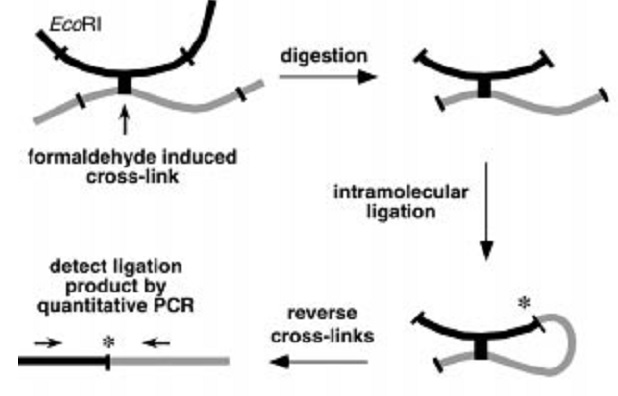
\includegraphics[scale=0.3]{3Cschematic}
\end{figure}
\end{frame}

\subsection{The experimental Data}\label{subsection_theExperimentalData}
\begin{frame}{The experimental data}
\begin{itemize}
\item Two replicate of the CC experiments were conducted by Nora et. al 2012. 
\item we focus on a 920,432 bp subset of the data, around the X inactivation center of the X chromosome in mouse embryonic stem cells. 
\item the region harbors the Xist enhancer and Tisx promoter.
\item we have the segments' encounter frequencies from the two experimental replicates.
\end{itemize}
\end{frame}

\begin{frame}{Topologically Associating Domains (TADs)}
Conserved structures of chromosome interactions on the Mb scale, with higher inter than intra-segment interactions
It is believed that the TAD forms a 'regulatory unit' for regulating gene expression, as can be seen by the correlation of gene expression located on the same TAD
\centering
\begin{figure}[H]

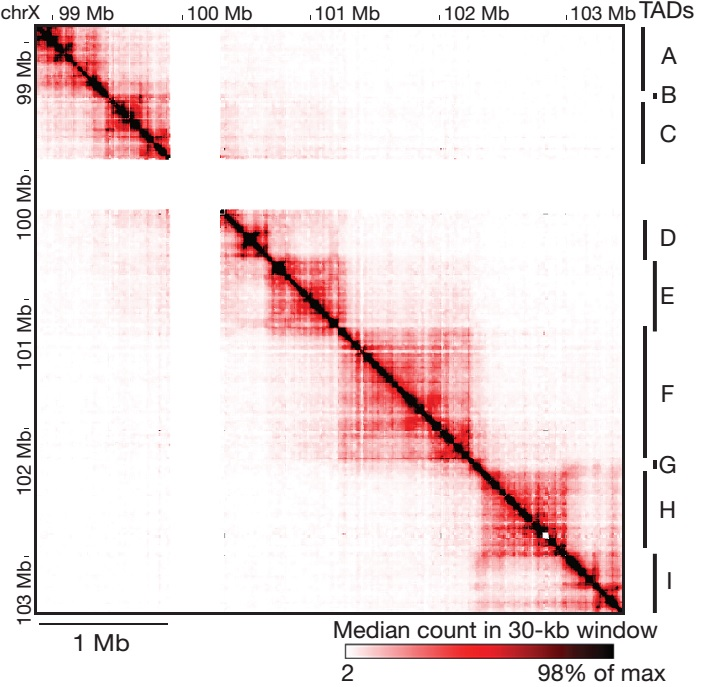
\includegraphics[scale=0.2]{TADsOfTheXChromosome_NoraEtAl2012}
\quad
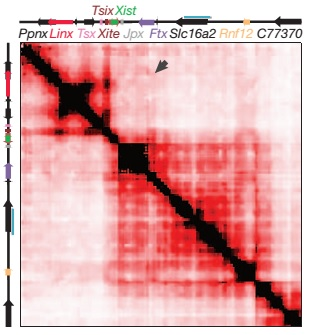
\includegraphics[scale=0.25]{TadDandENoraEtAl2012} 
\quad
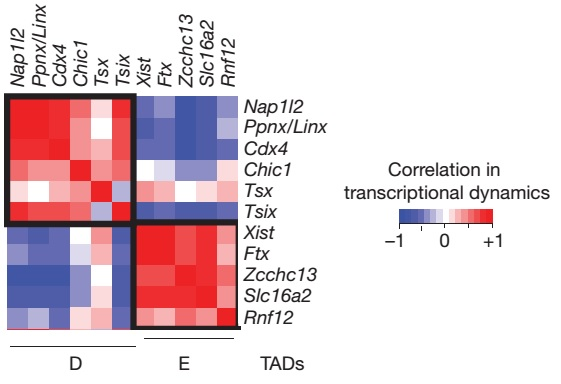
\includegraphics[scale=0.27]{transcriptionCorrelationTadDandENoraEtAl2012}
\caption{\tiny{The 4.5 Mb region (left), enlargement of TAD D and E (center). Displayed median count in a 30kb window every 6kb, gene expression correlation (right)}}
\label{fig:TADsOfTheXChromosome_NoraEtAl2012}
\end{figure}
\end{frame}

\section{Analysis of the data}\label{section_analysisOfTheData}
\begin{frame}{From restriction segments to beads}
\begin{itemize}
\item To coarse-grain the data, we choose a bead-size of 3000 bp, corresponding to the mean segment length resulted from the digestion of EcoRIII enzyme. 

\begin{figure}[H]
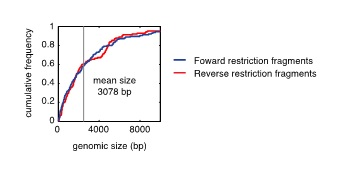
\includegraphics[scale=0.55]{restrictionSegmentLengthDistributionLucaetal}
\end{figure}
\item the genomic section was evenly partitioned by 3000 bp beads. Each segment receives a start and end index according to the beads it covers. 
\item for example, 
\begin{tabular}[H]{|l| l| l|}
\hline
bp range & start ind & end ind\\
\hline
500-3500   & 1         & 2 \\
4000-4500  & 2         & 2 \\   
5000-12001 & 2         & 4 \\       
\hline  
\end{tabular}
\end{itemize}
\end{frame}


\subsection{TAD D and E}\label{subsection_tadDAndE}
\begin{frame}{Bead encounter frequecy}
\framesubtitle{TAD D and E}
\begin{itemize}
\item We work with the average of the two experimental replicates
\item a total length of 920,432 bp - resulting in 307 beads (TAD D 107 beads, TAD E 200 beads)
\item We calculate the 'one-sided' encounter probability vs. distance (bead units) for each bead
\item the mean encounter probability difference, shows that the data is left-right symmetric

\begin{figure}[H]
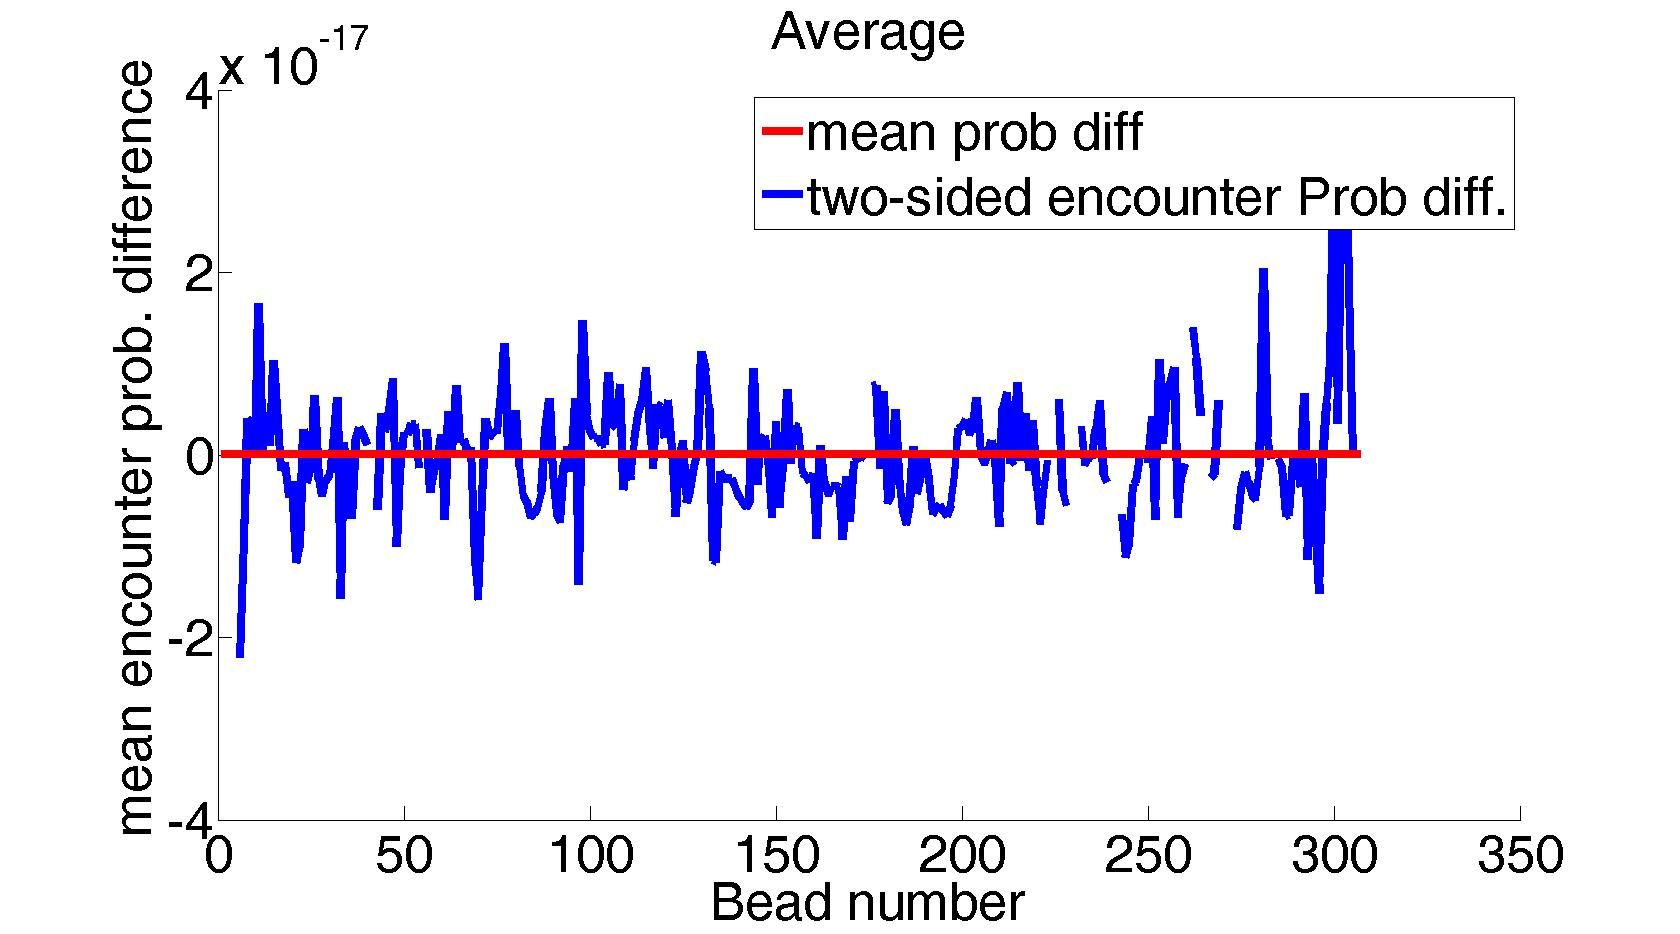
\includegraphics[scale=0.05]{symmetryOfTheEncounterProbability307BeadsAverage}
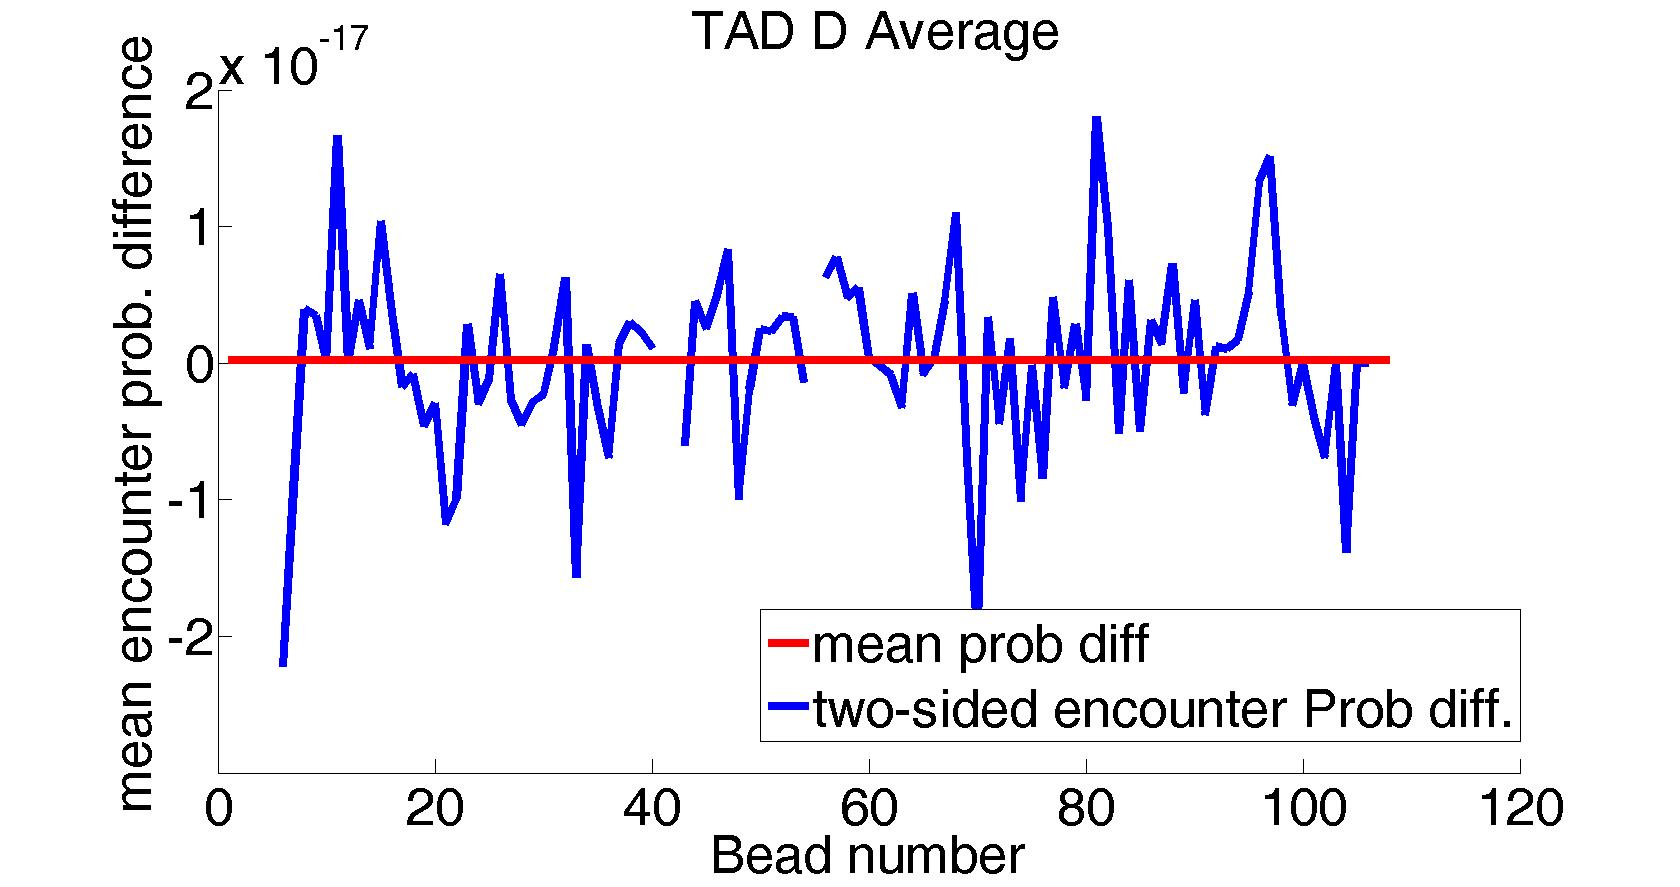
\includegraphics[scale=0.05]{symmetryOfTheEncounterProbabilityTADDAverage}
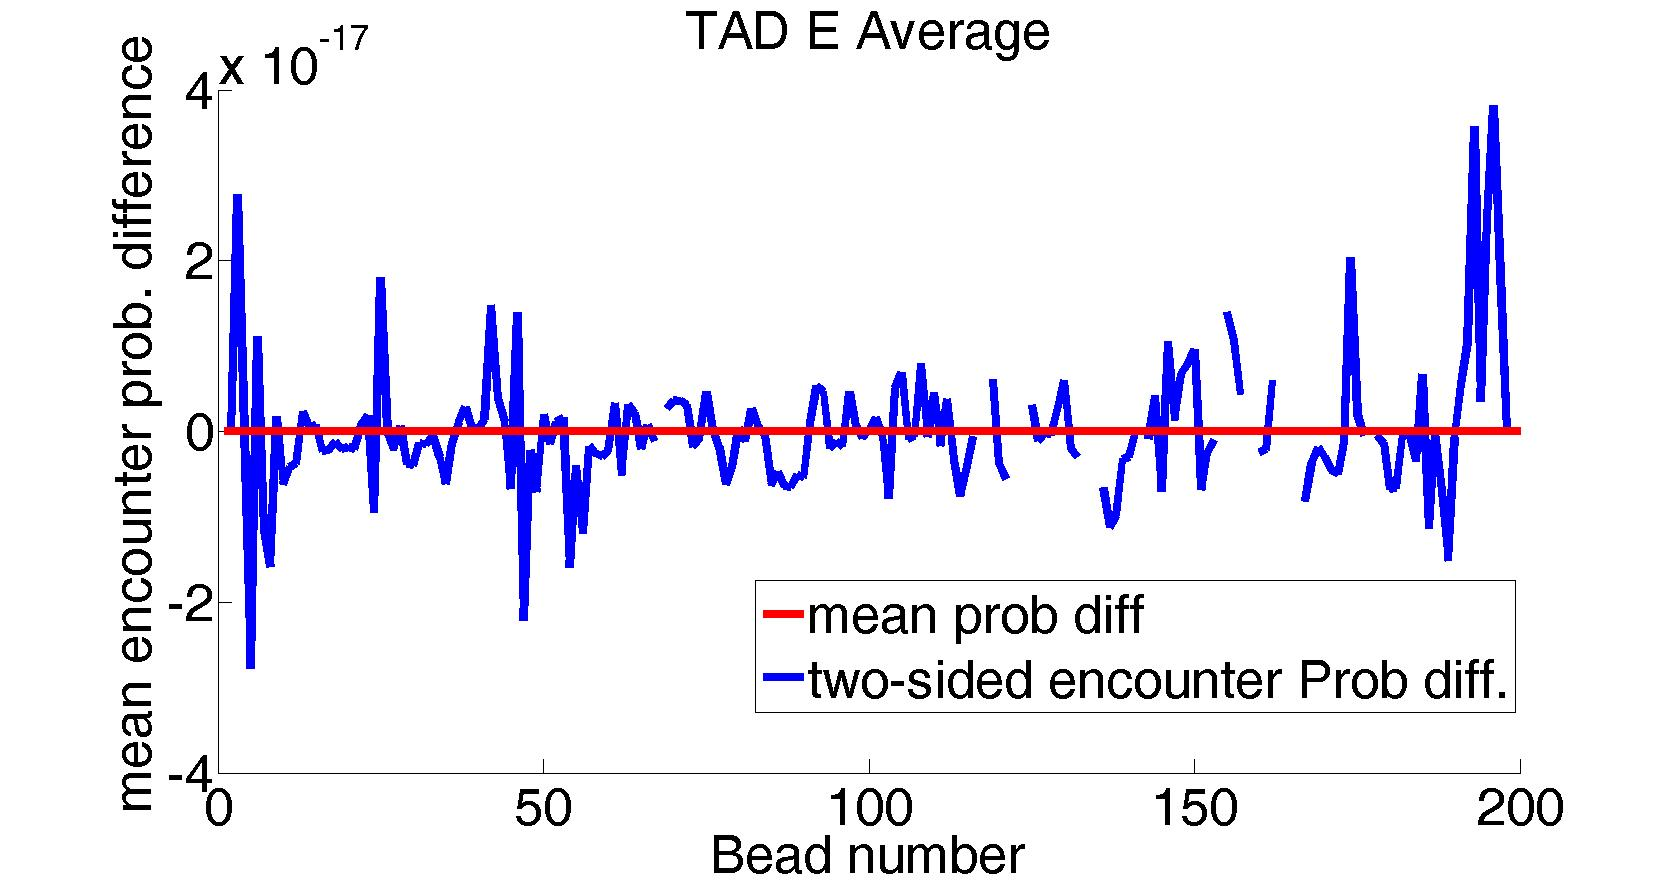
\includegraphics[scale=0.05]{symmetryOfTheEncounterProbabilityTADEAverage}
\end{figure}
\item TAD E has several strong specific interactions. TAD D has almost no specific interactions. Strong inter-TAD specific interactions
\end{itemize}

\begin{figure}[H]\label{TADDAndEencounterProb}
\centering
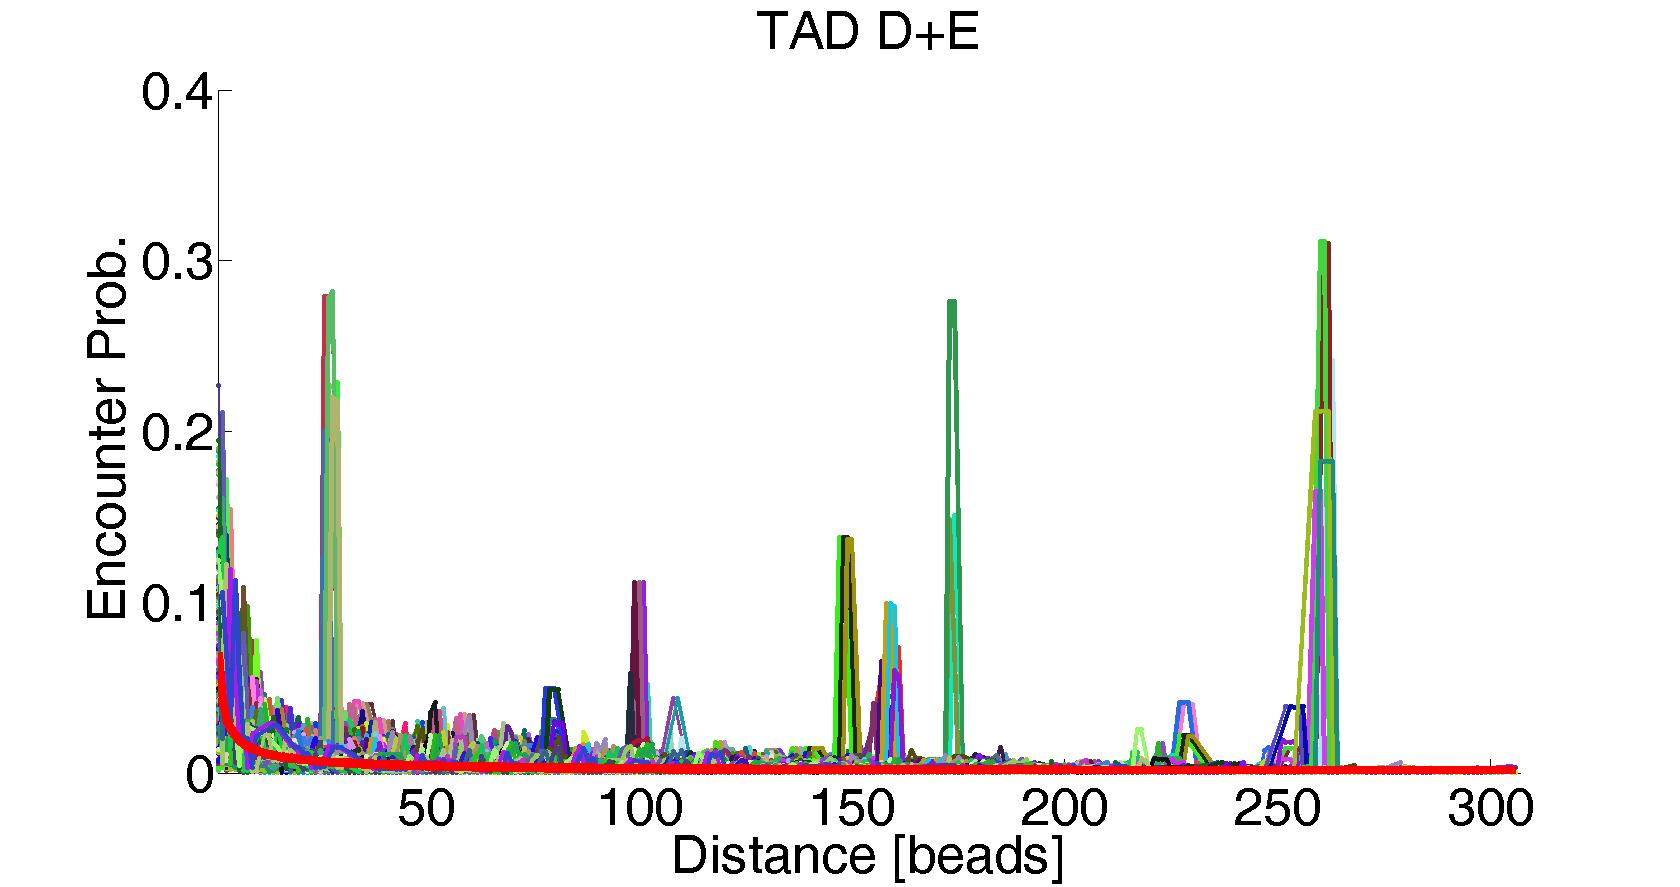
\includegraphics[scale=0.078]{encounterProbabilityTADDAndE}
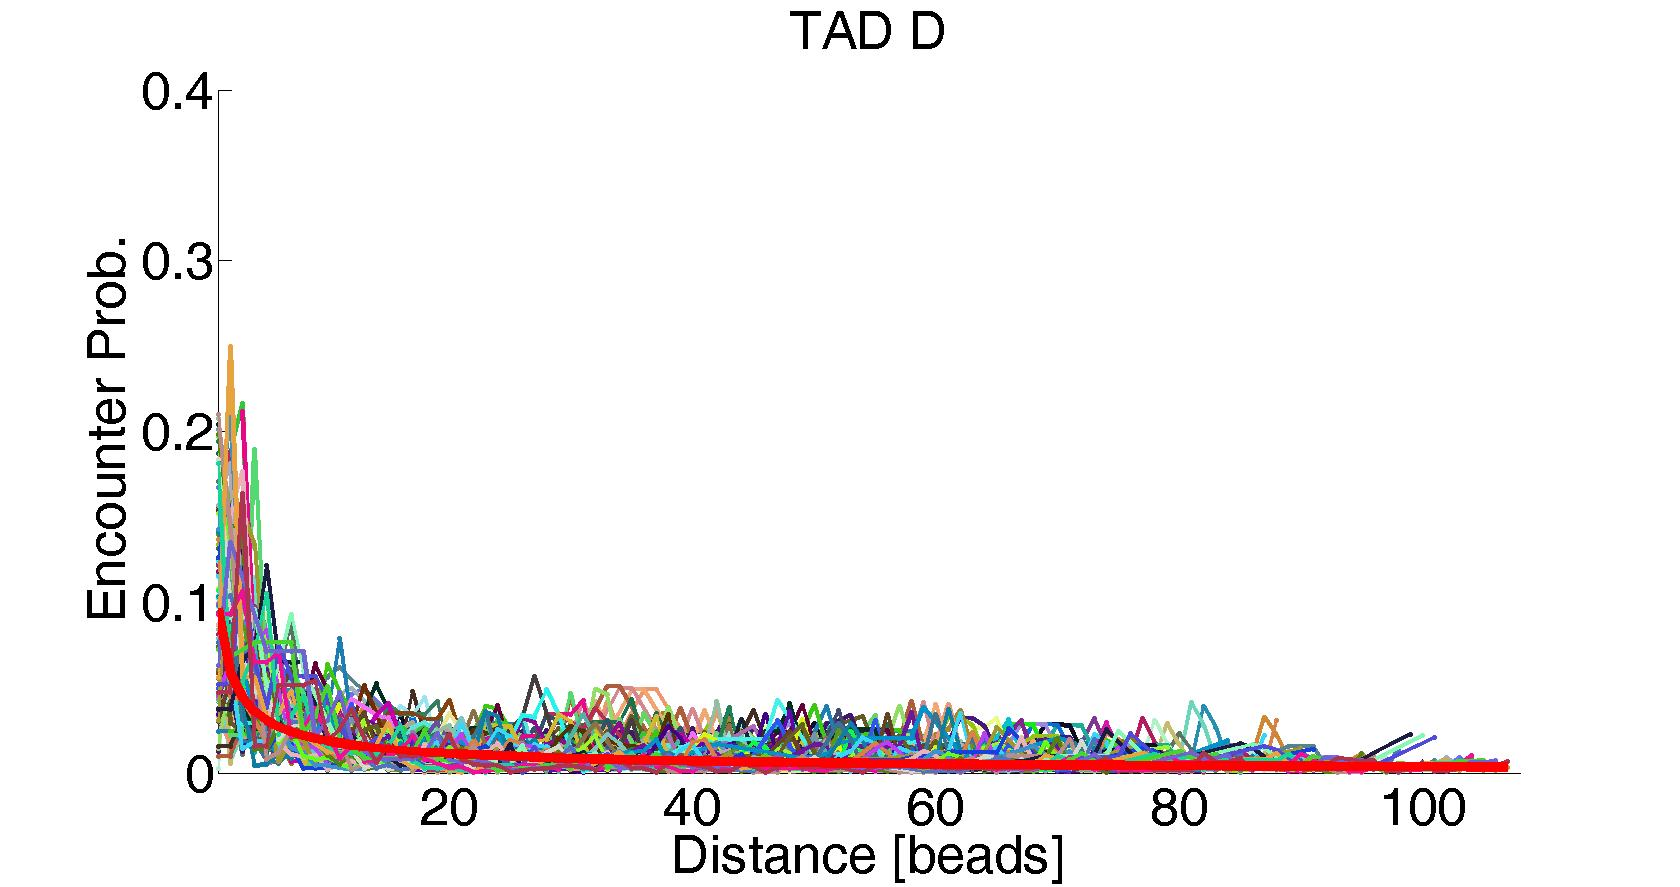
\includegraphics[scale=0.075]{encounterProbabilityTADD}
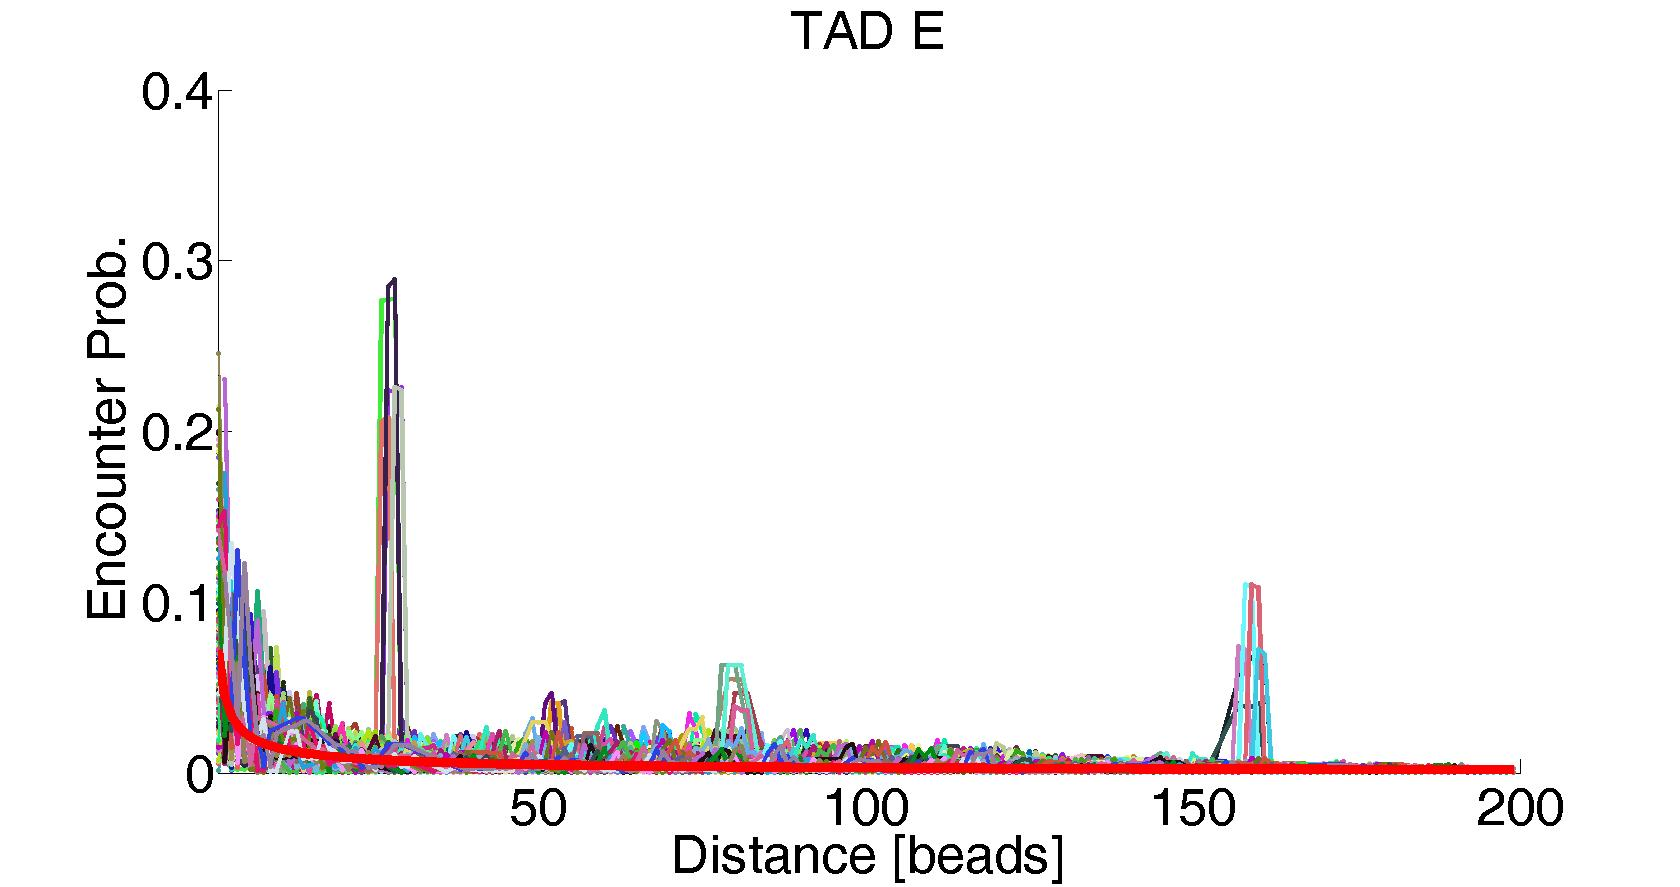
\includegraphics[scale=0.075]{encounterProbabilityTADE}
\end{figure}
\end{frame}

\subsection{Peaks of the encounter data}
\begin{frame}{Peaks of the encounter data}
\begin{itemize}
\item About half of the peaks in the encounter data result from specific interactions \textcolor{red}{between TADs}
\item The other half comes from specific internal interactions of \textcolor{green}{TAD E}.
\item To get an impression, a manual marking of the peaks shows 
\end{itemize}
\begin{table}[H]\label{nonNeighborBeadEncounterTable}
\begin{tabular}{l l l}
Bead numbers & Encountered beads & TAD\\
\hline
23-26   & 280-290 & \textcolor{red}{$D\leftrightarrow E$}\\
49-53   & 148-155 & \textcolor{red}{$D\leftrightarrow E$}\\
56-59   & 80-90   & $D\leftrightarrow D$\\
115-117 & 165-170 & \textcolor{green}{$E\leftrightarrow E$}\\
161-162 & 187 190 & \textcolor{green}{$E\leftrightarrow E$}\\
182-184 & 260-264 & \textcolor{green}{$E\leftrightarrow E$}\\
185-186 & 253-255 & \textcolor{green}{$E\leftrightarrow E$}\\
234-236 & 184-189 & \textcolor{green}{$E\leftrightarrow E$}\\
234-236 & 4-11    & \textcolor{red}{$E\leftrightarrow D$}\\
243     & 88      & \textcolor{red}{$E\leftrightarrow D$}\\
264     & 89-90   & \textcolor{red}{$E\leftrightarrow D$}\\
274-277 & 113-120 & \textcolor{green}{$E\leftrightarrow E$}
\end{tabular}
\end{table} 
\end{frame}

\subsection{The encounter probability}\label{subsection_theEncounterProbability}
\begin{frame}{The enconter probability}
For the case of TAD D, TAD E, and the two together, we estimate the bead encounter probability, $p$, and fit it with a function of the form 
\begin{equation*}
p_n(d)=\alpha d^{-\beta}
\end{equation*}
where, $d$ is the distance in bead units, $\alpha=\frac{1}{\sum_{j=1}^{d_{max}}j^{-\beta}}$ and $\beta$ is a parameter to be estimated.
We report the values of $\beta$ for each bead in each case
\begin{figure}[H]
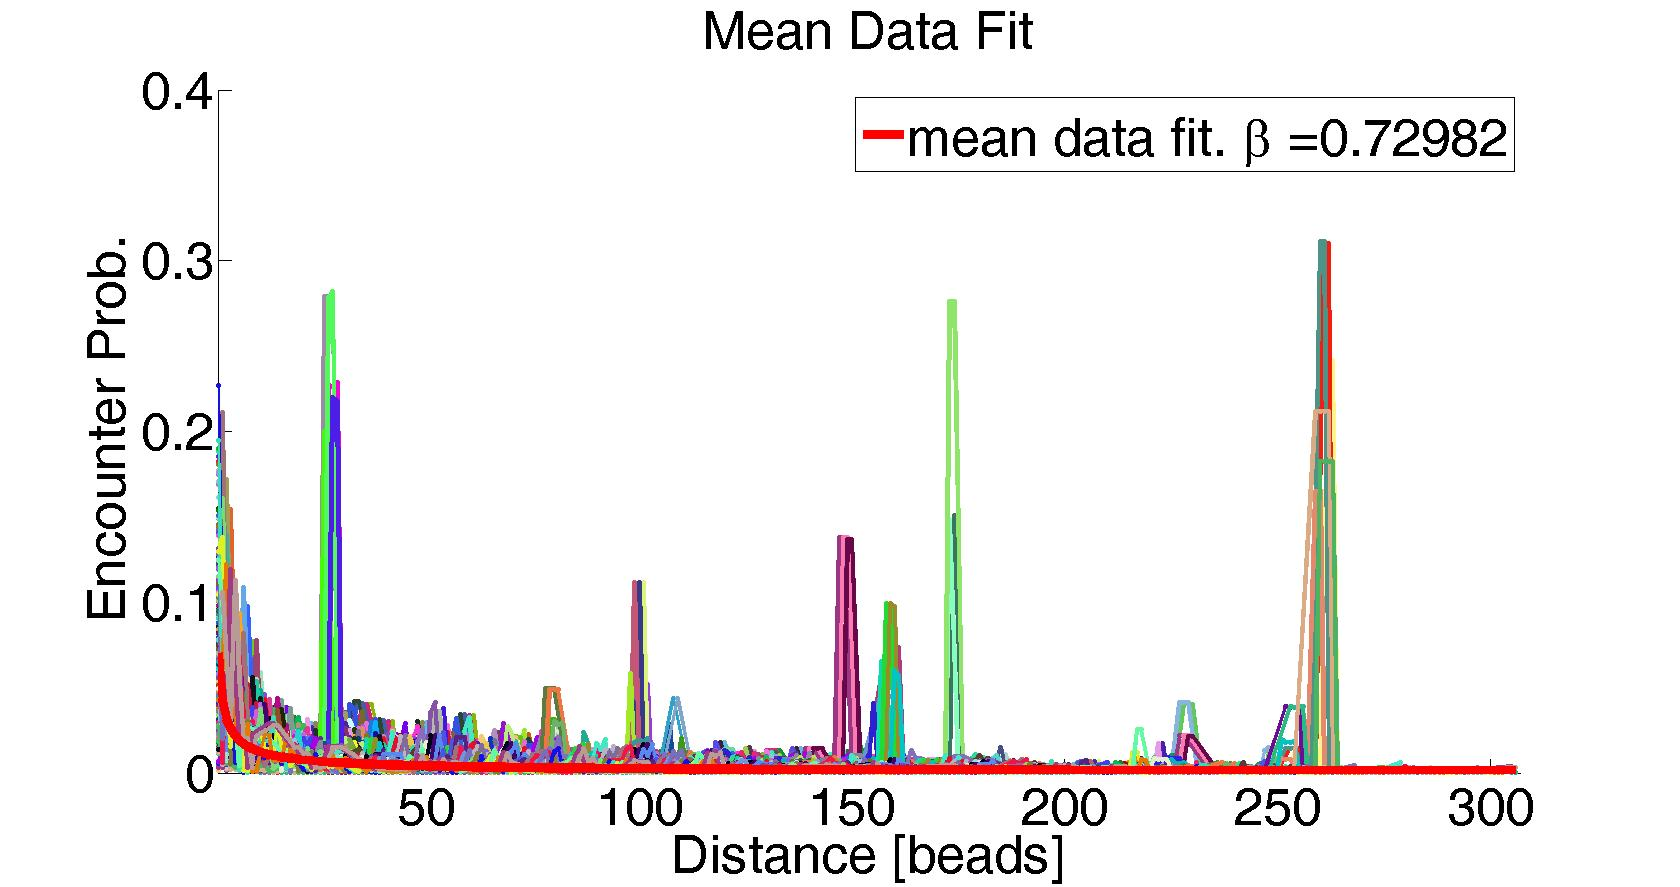
\includegraphics[scale=0.1]{meanDataFitTADDAndE}
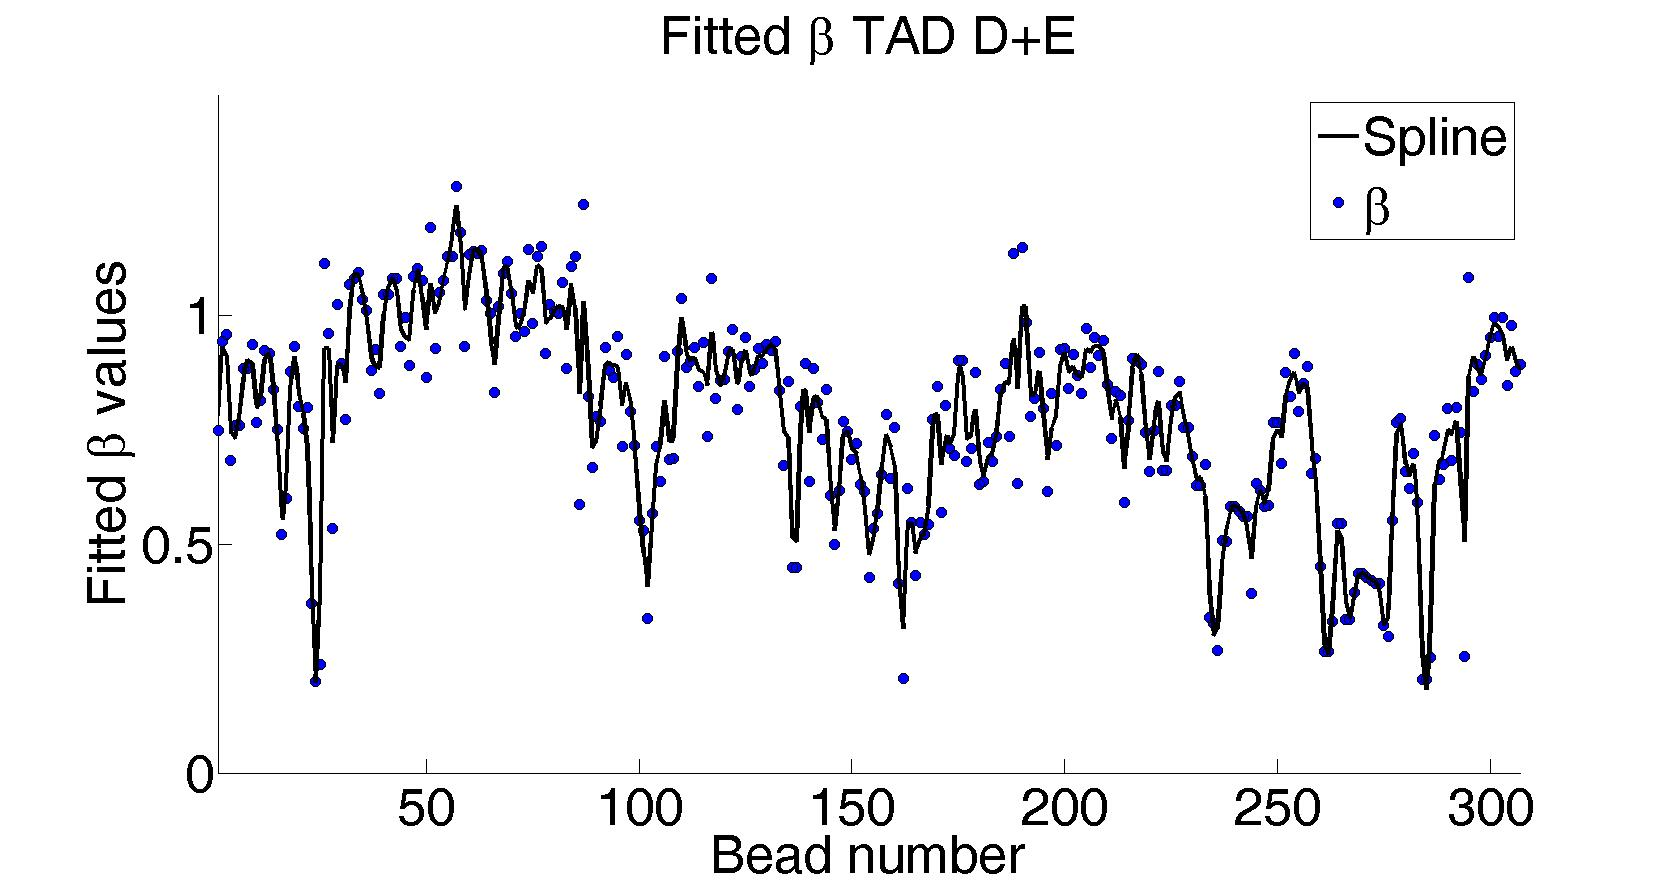
\includegraphics[scale=0.1]{fittedExpValuesWithSplineAverageTADDAndE}
\end{figure}
\end{frame}

\begin{frame}
\framesubtitle{TAD D and E}
\begin{figure}[H]
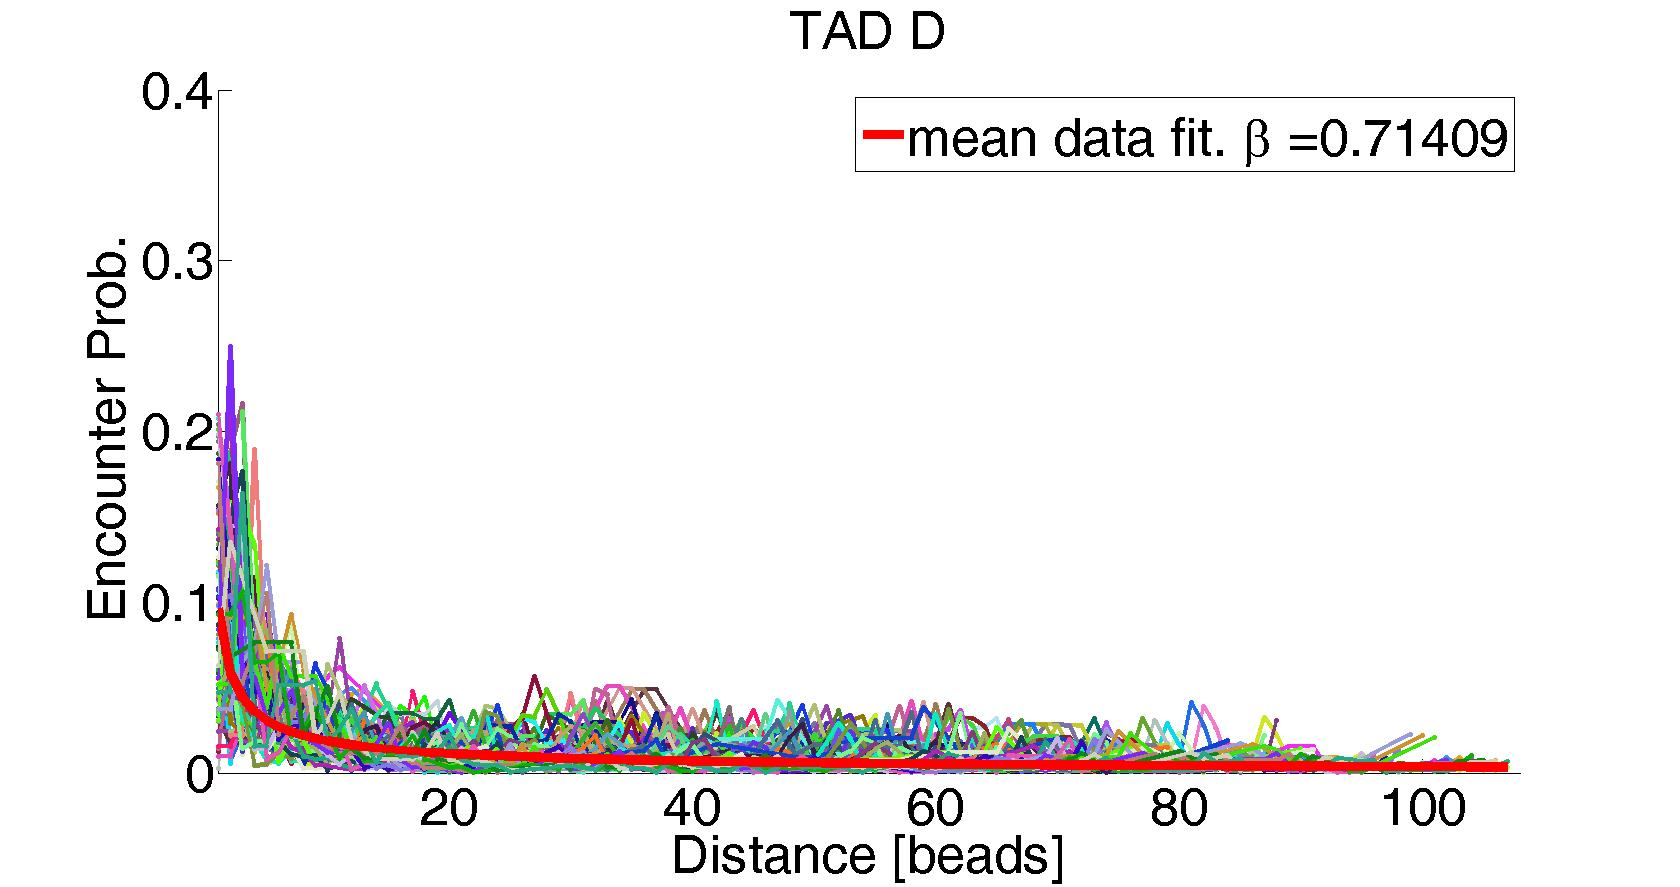
\includegraphics[scale=0.1]{meanDataFitTADD}
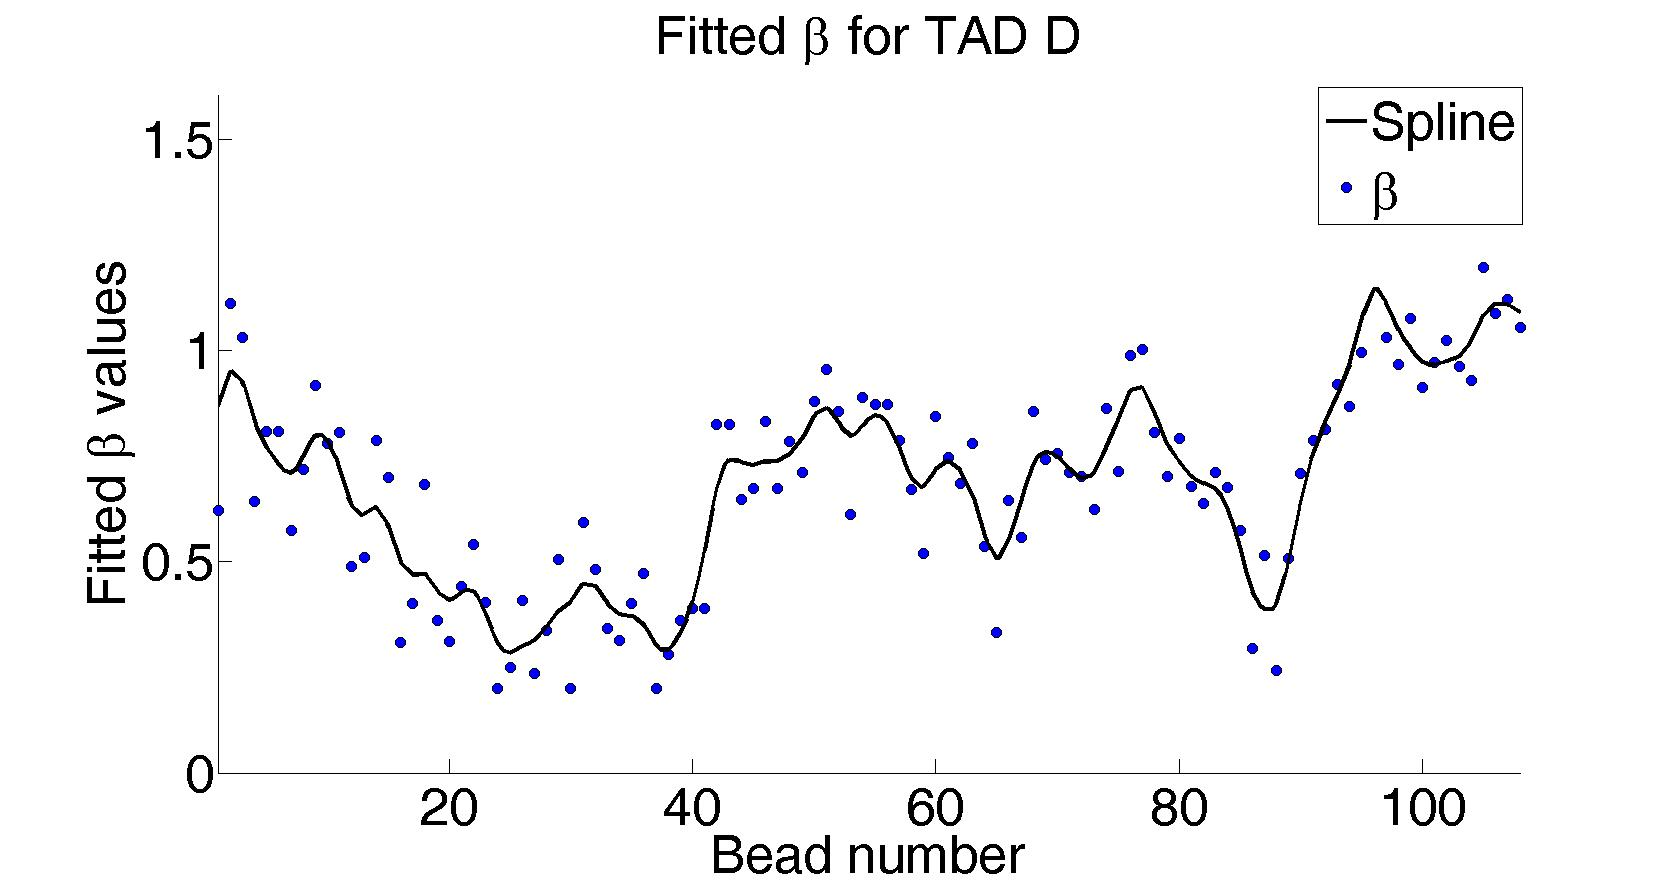
\includegraphics[scale=0.1]{fittedExpValuesWithSplineAverageTADD}
\end{figure}

\begin{figure}[H]
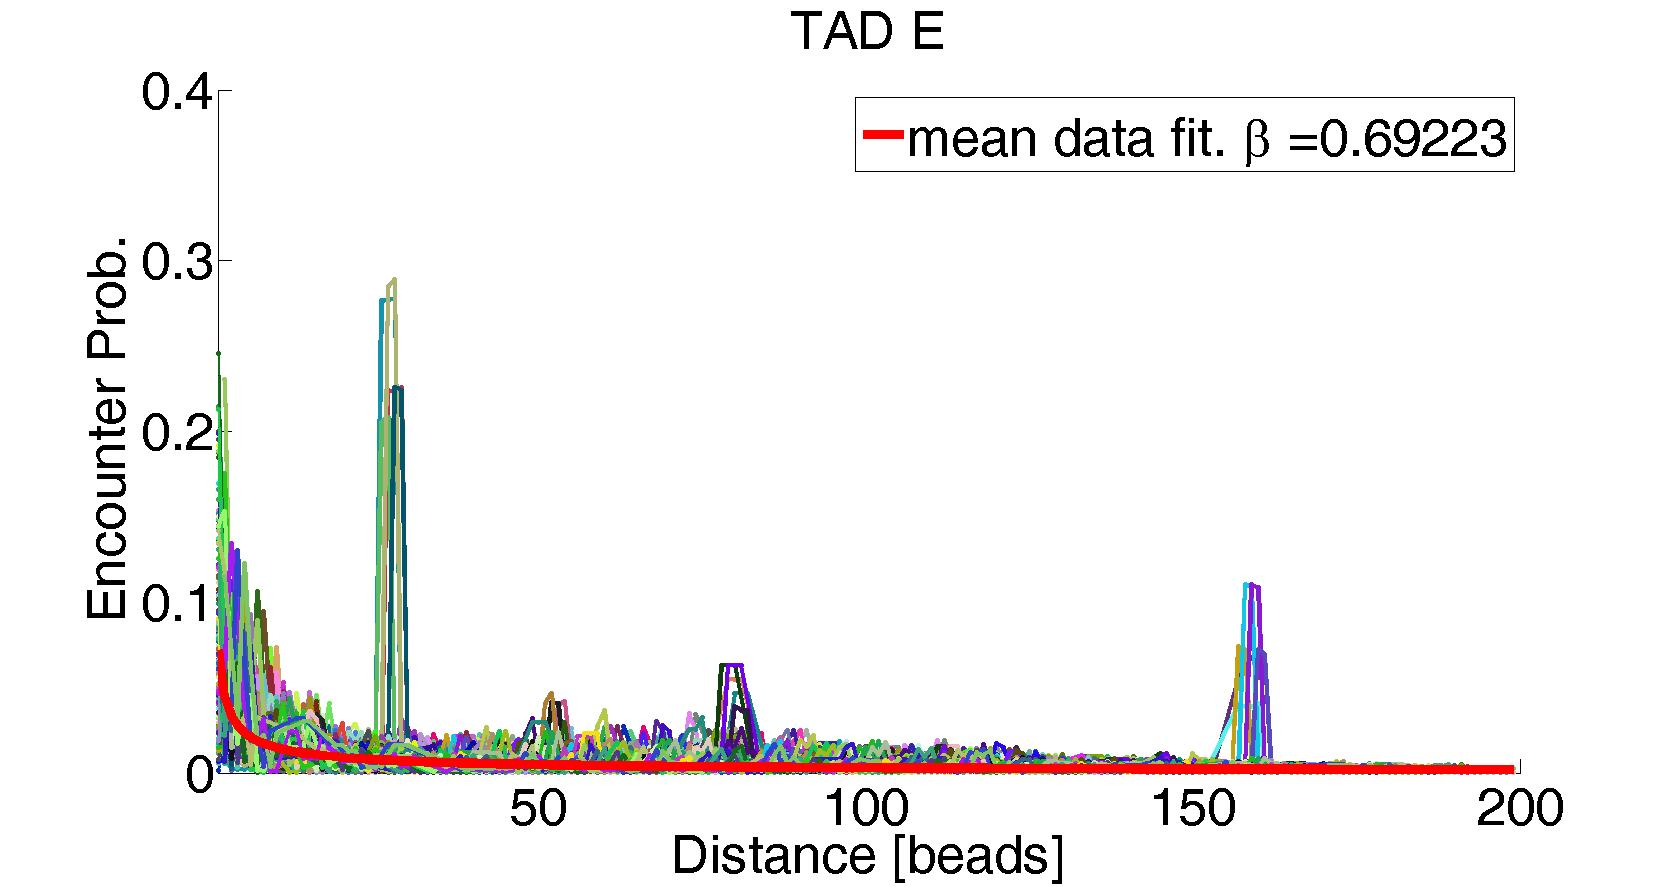
\includegraphics[scale=0.1]{meanDataFitTADE}
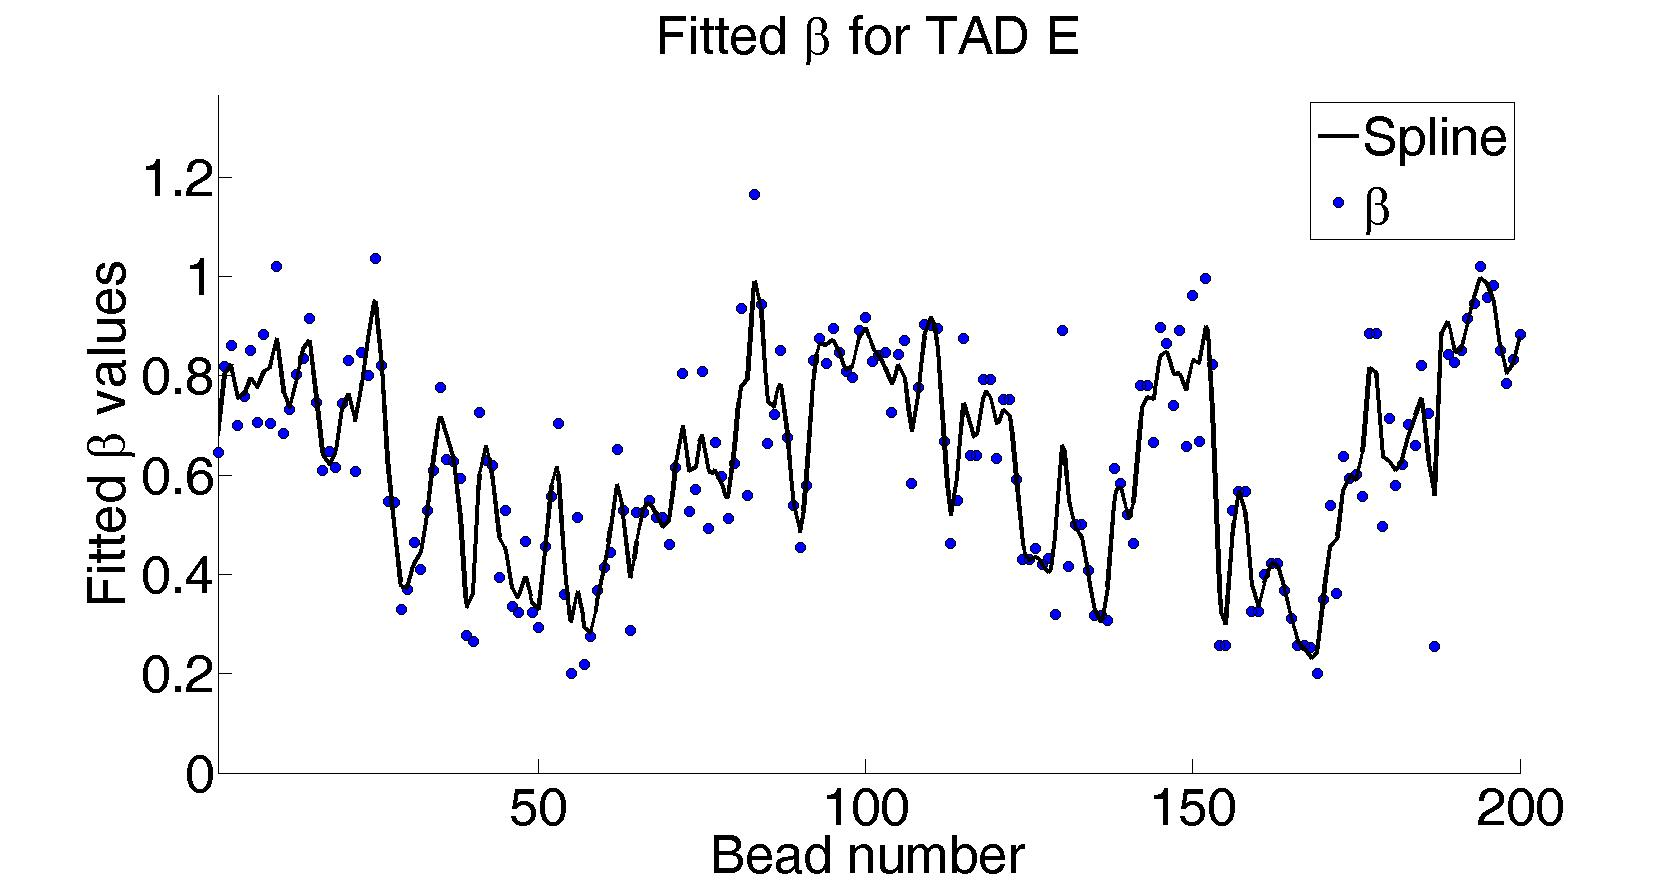
\includegraphics[scale=0.1]{fittedExpValuesWithSplineAverageTADE}
\end{figure}


\end{frame}
\section{Theoretical model}\label{section_theoreticalModel}
\begin{frame}{Theoretical model}
\framesubtitle{The Rouse model}
We start with the classical and most simple model, the Rouse chain.
\begin{itemize}
\item A Rouse chain describes polymer dynamics as a stochastic motion of a collection of microscopic "beads" connected by harmonic springs
\item the 3D  motion of bead $n$ in the chain of $N$ beads 
\begin{equation*}
\frac{dR_n}{dt} = -\frac{3D}{b^2}(2R_n(t)-R_{n+1}(t)-R_{n-1}(t))+f_n(t)
\end{equation*}
\item $R_n$- the position of bead $n$\\
$b$- the standard deviation of the distance between adjacent beads\\
$D$- the diffusion constant\\
$f_n$- white Gaussian noise
\item From the theory, $Pr(\|R_n-R_m\|<\epsilon)\sim  |n-m|^{-1.5}$
\end{itemize}
\end{frame}

\section{Simulation Results}\label{section_simulationResults}
%simulation section order:
% 1. normal Rouse 
% 2. normal rouse with peaks
% 3. rouse with random loops one TAD with tails 
% 4. rouse with random fixed loops in two TADs

\subsection{Simulations with a simple rouse chain}
\begin{frame}{Simulation with simple rouse chain}
\begin{itemize}
\item A simple Rouse model cannot reproduce the TAD, as expected.
\item placing loops corresponding to the peaks of the encounter data does not reproduce the TADs. 
\end{itemize}
\begin{figure}[H]
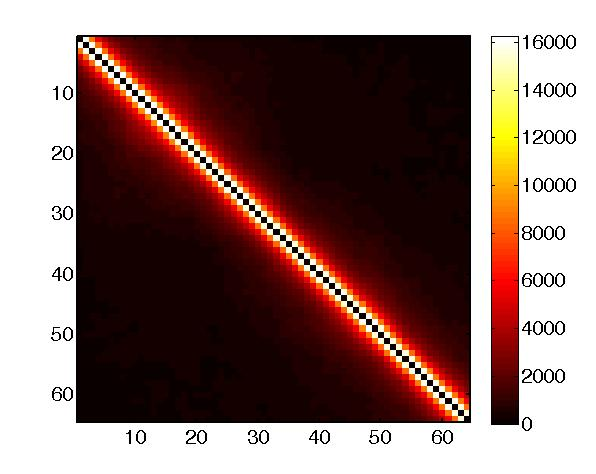
\includegraphics[scale=0.17]{encounterMatrix64Beads}
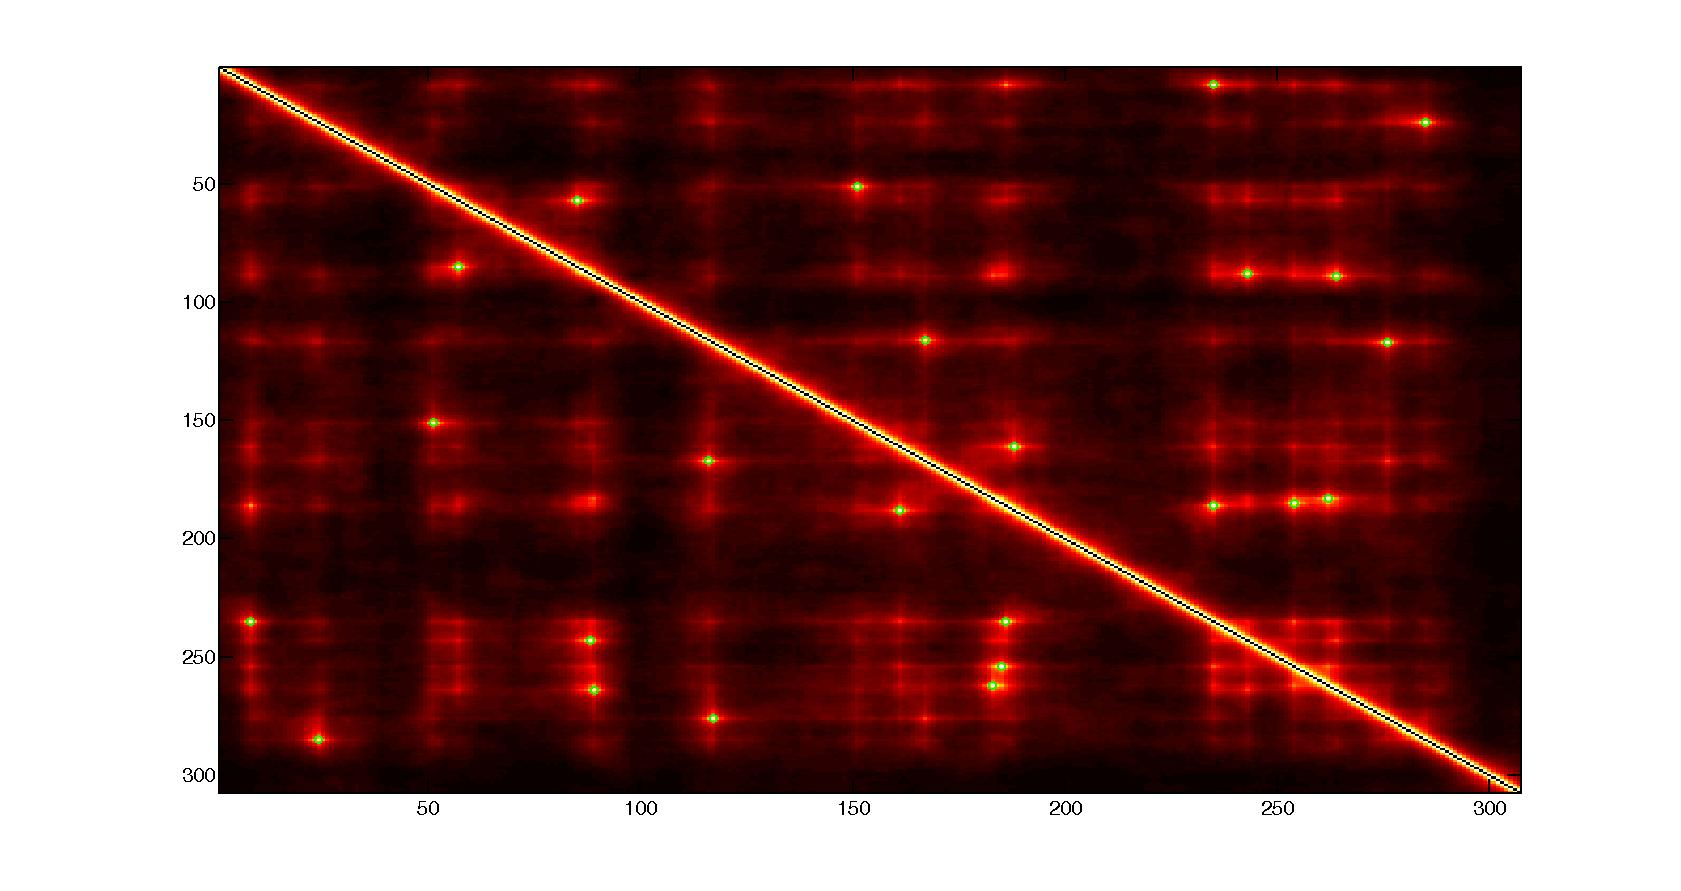
\includegraphics[scale=0.09]{meanEncounterMatrixOfSimulatingTADEandDWithLoops}
\end{figure}
\end{frame}

\subsection{Random loops model}\label{subsection_randomLoopsModel}
\begin{frame}{Random Fixed Loop Model}
\begin{itemize}
\item The enhancer-transcription factor elements' encounter motivates the simulation of a chain with randomly placed loops
\item these encounters might not be as frequent as 'stable' loops in the chromatin and therefore not shown significantly in the encounter maps
\item simulate a chain of 64 beads, having a random loop in a bounded genomic region
\item increasing number of loops at random position is simulated 
\end{itemize}

\end{frame}

\begin{frame}{Random loops in a bounded region}
\framesubtitle{One TAD}
We examine the behavior of the encounter probability when we restrict the loops to be in one region of the polymer, increasing the number of loops from 1 to 8.
\begin{figure}[H]
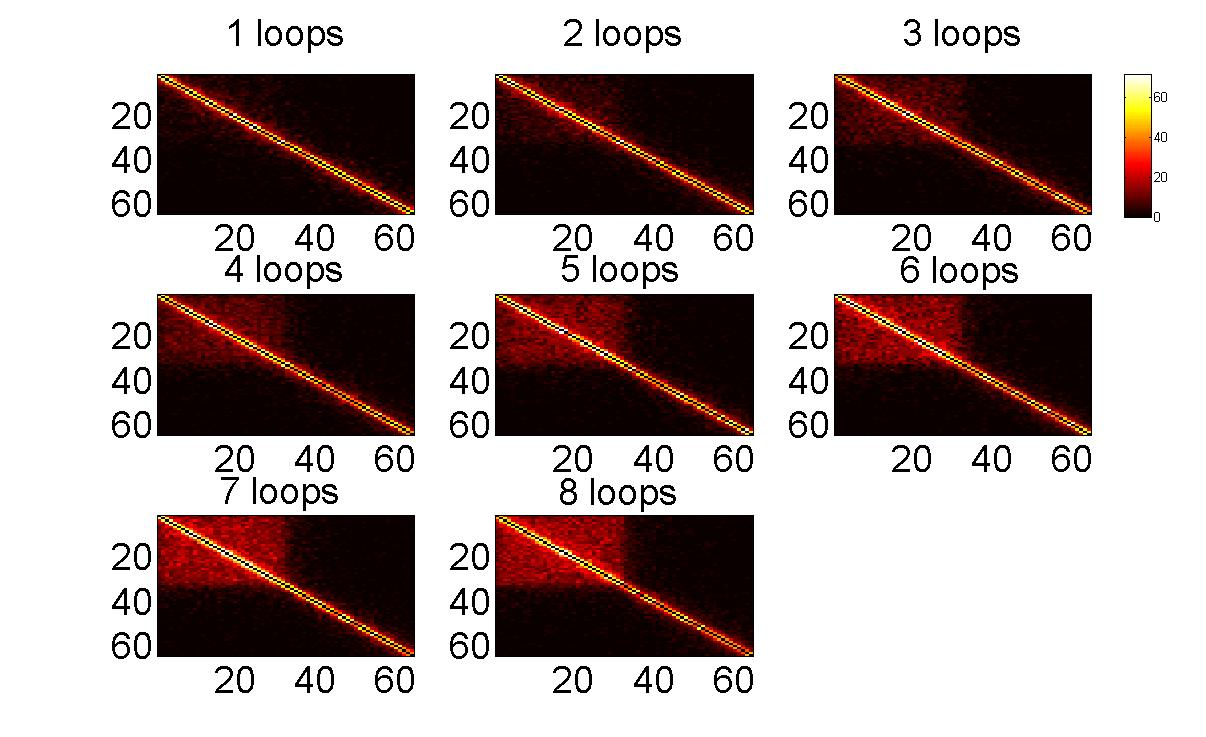
\includegraphics[scale=0.13]{encounterHistogramOneTAD_1to8Loops}
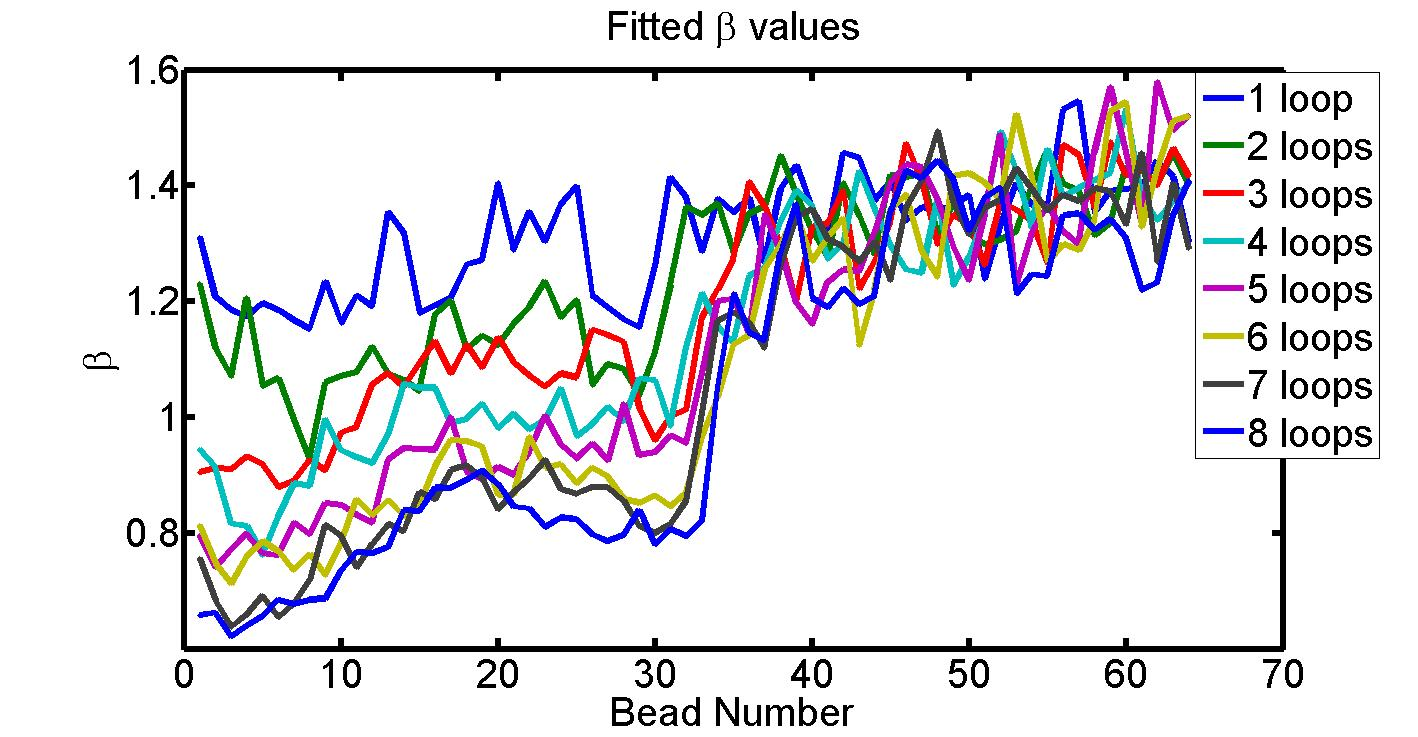
\includegraphics[scale=0.13]{fittedExpOneTAD1To8Loops}
\end{figure}
\end{frame}


\begin{frame}{Random loops in a bounded region}
\framesubtitle{Two TADs}
The same can be done with two bounded regions, where the number of loops is increased from 1 to 10 in a 64 beads chain. 
\begin{figure}[H]
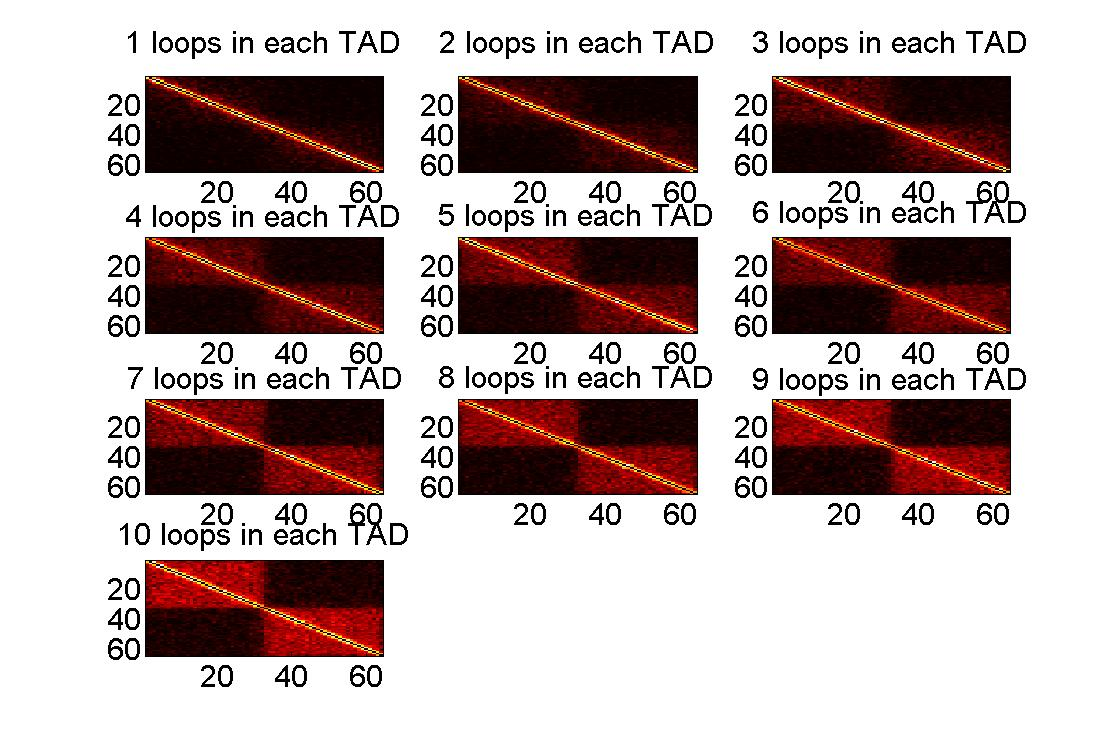
\includegraphics[scale=0.15]{encounterHistogram1To10LoopsInEachTAD}
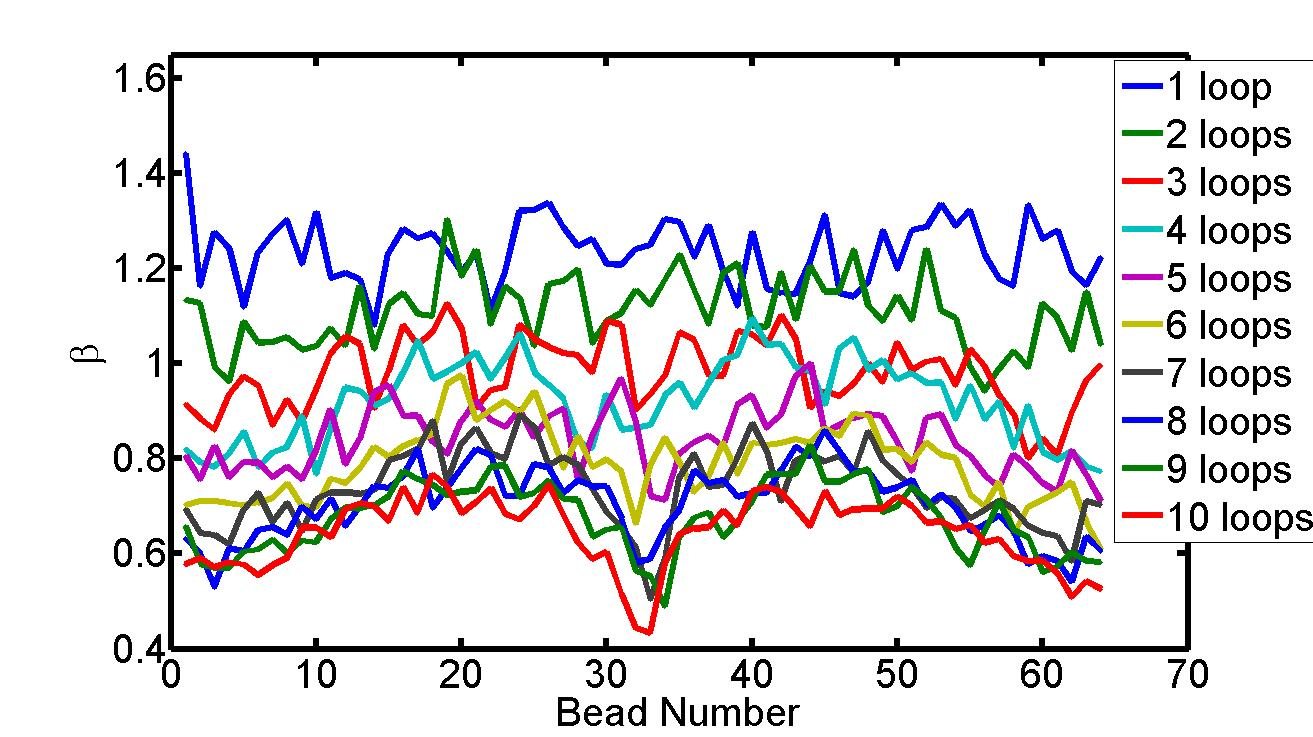
\includegraphics[scale=0.13]{fittedExpTwoTADs1To10Loops}
\end{figure}
\end{frame}

\subsection{Peaks in the periphery of TADs}\label{subsection_peaksInThePeripheryOfTADs}
\begin{frame}{Peaks at the edges of TADs}
At the edges of TADs there are significant peaks of the encounter frequencies.
The encounter data of Nora et al. was smoothed using a median filter therefore, those peaks where not shown clearly.
Such peaks might indicate a stable loop in the structure of the genomic region and should be taken into account.

\begin{figure}[H]
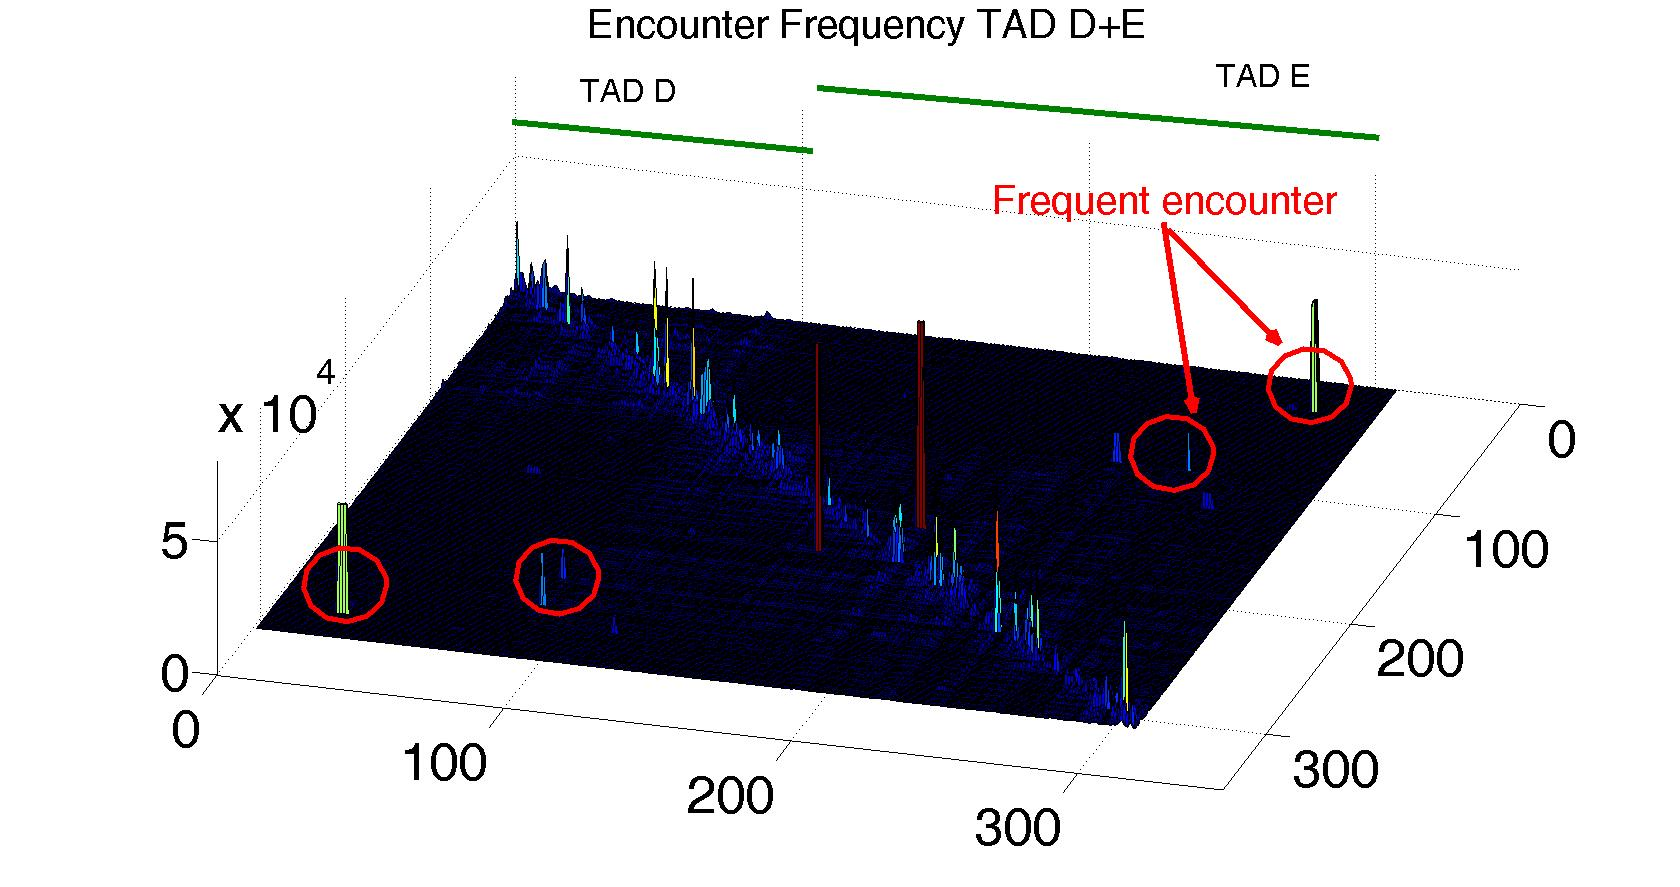
\includegraphics[scale=0.2]{peaksOfTADDAndEInSurfPlot}
\end{figure}
\end{frame}

\begin{frame}{Stable loop with random loops within}
\framesubtitle{one TAD with 'tails'}
\begin{enumerate}
\item Following the peaks observation, we form a mix of 'stable' big loop with internal random loops
\item in a 64 beads chain, beads 15 and 50 were connected
\item we iteratively add 11 loops within the stable loop
\item we can start seeing the emergence of $\beta$ curve pattern as in the experimental data
\end{enumerate}
\begin{figure}[H]
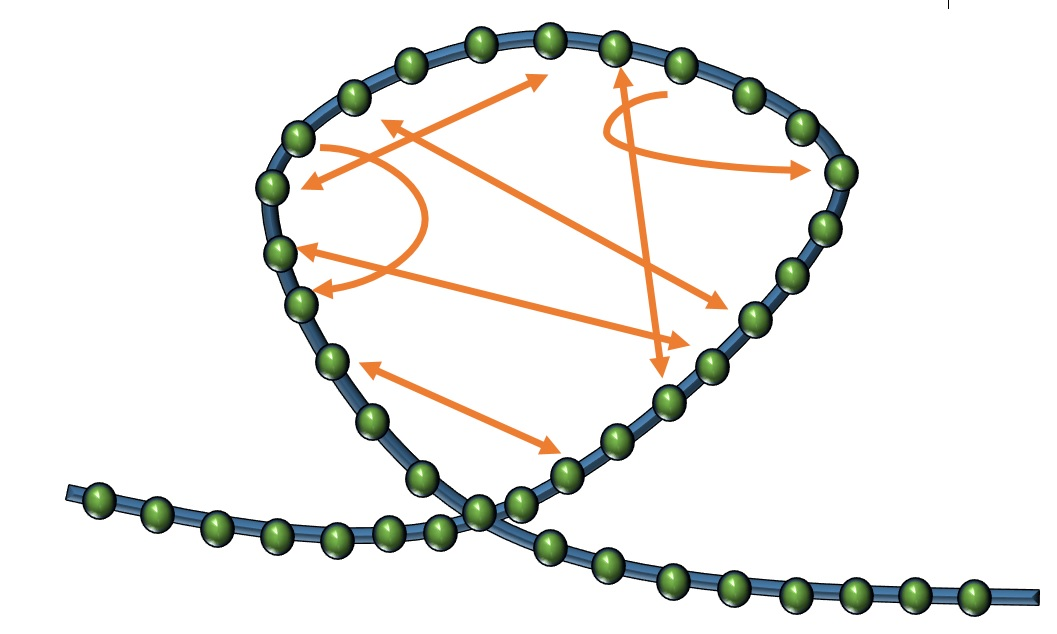
\includegraphics[scale=0.06]{polymerModelWithLoopAndInternalConnectors}
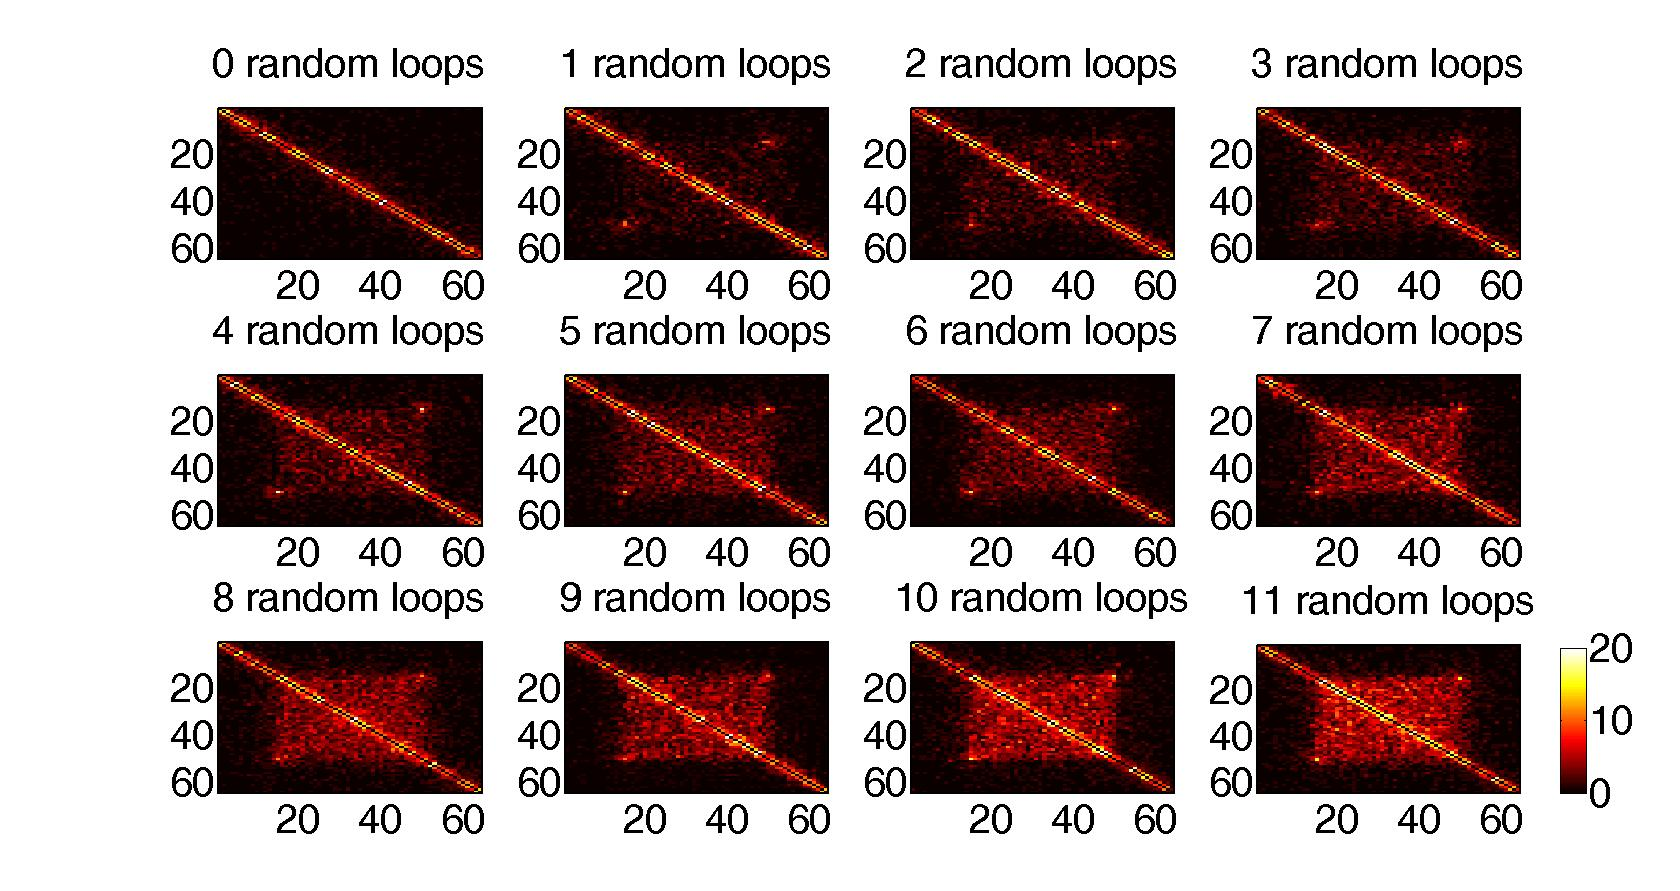
\includegraphics[scale=0.08]{encounterHistogram_randomInternalLoops64BeadChain}
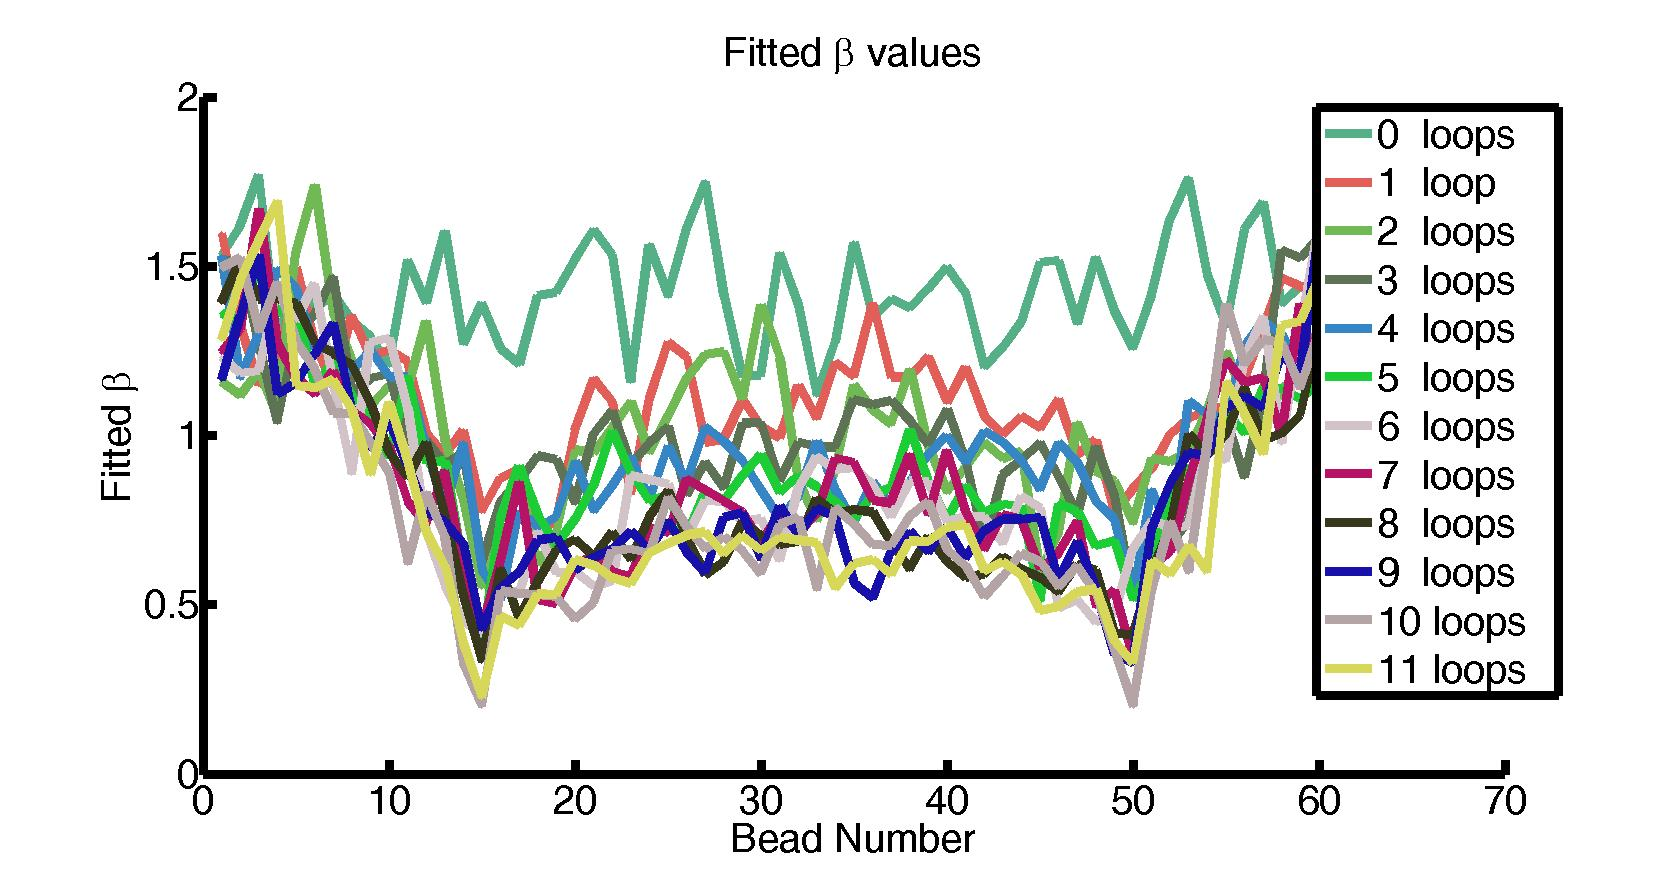
\includegraphics[scale=0.08]{fittedExpOneTADWithTails64Beads1To11Loops}
\end{figure}
\end{frame}

\subsection{$\beta$ as a function of the number of loops}\label{subsection_betaAsAFunctionOfTheNumberOfLoops}
\begin{frame}{$\beta$ as a function of the number of loops}
\begin{enumerate}
\item Through simulation we observe a quadratic relationship between the mean fitted $\beta$ value and the number of random loops
\item this enables us to say something about the mean structure
\item the mean number of loops in a given genomic region can be extracted from experimental data
\end{enumerate}
\begin{figure}[H]
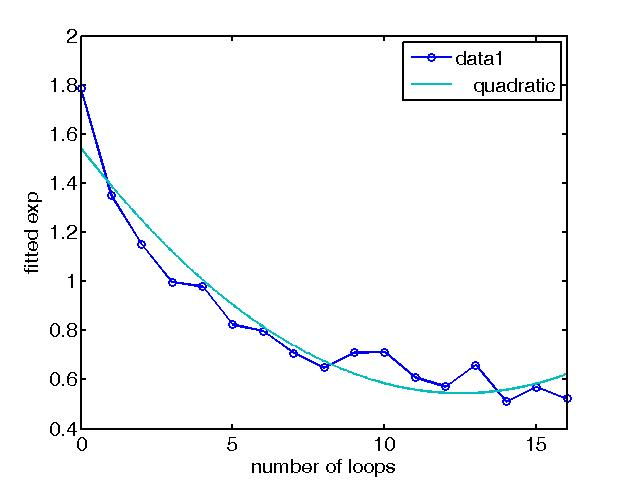
\includegraphics[scale=0.2]{changeOfExponentAsAfunctionOfLoopsStableLoopModelVariableLoops32Beads}
\end{figure}
\end{frame}

\subsection{Literature on random loops}
\begin{frame}{Literature supprt for random enhancer promoter interactions}
\scriptsize{
\begin{enumerate}
\item Job Dekker, Marc A Marti-Renom, and Leonid A Mirny. Exploring
the three-dimensional organization of genomes: interpreting chromatin
interaction data. Nature Reviews Genetics, 14(6):390–403, 2013
\item Job Dekker, Karsten Rippe, Martijn Dekker, and Nancy Kleckner. Capturing chromosome conformation. science, 295(5558):1306–1311, 2002.
\item Jos´ee Dostie, Todd A Richmond, Ramy A Arnaout, Rebecca R Selzer,
William L Lee, Tracey A Honan, Eric D Rubio, Anton Krumm, Justin
Lamb, Chad Nusbaum, et al. Chromosome conformation capture carbon
copy (5c): a massively parallel solution for mapping interactions between
genomic elements. Genome research, 16(10):1299–1309, 2006
\item Peter Fraser and Wendy Bickmore. Nuclear organization of the genome
and the potential for gene regulation. Nature, 447(7143):413–417, 2007
\item Johan H Gibcus and Job Dekker. The hierarchy of the 3d genome.
Molecular cell, 49(5):773–782, 2013
\item Suchit Jhunjhunwala, Menno C van Zelm, Mandy M Peak, Steve
Cutchin, Roy Riblet, Jacques JM van Dongen, Frank G Grosveld, Tobias A Knoch, and Cornelis Murre. The 3d structure of the immunoglobulin heavy-chain locus: implications for long-range genomic interactions.
Cell, 133(2):265–279, 2008
\item Erez Lieberman-Aiden, Nynke L van Berkum, Louise Williams, Maxim
Imakaev, Tobias Ragoczy, Agnes Telling, Ido Amit, Bryan R Lajoie,
Peter J Sabo, Michael O Dorschner, et al. Comprehensive mapping of
long-range interactions reveals folding principles of the human genome.
science, 326(5950):289–293, 2009.
\item Erez Lieberman-Aiden, Nynke L van Berkum, Louise Williams, Maxim
Imakaev, Tobias Ragoczy, Agnes Telling, Ido Amit, Bryan R Lajoie,
Peter J Sabo, Michael O Dorschner, et al. Comprehensive mapping of
long-range interactions reveals folding principles of the human genome.
science, 326(5950):289–293, 2009.
\item Erez Lieberman-Aiden, Nynke L van Berkum, Louise Williams, Maxim
Imakaev, Tobias Ragoczy, Agnes Telling, Ido Amit, Bryan R Lajoie,
Peter J Sabo, Michael O Dorschner, et al. Comprehensive mapping of
long-range interactions reveals folding principles of the human genome.
science, 326(5950):289–293, 2009.
\end{enumerate}
}
etc..
\end{frame}

\section{Summary and future work}\label{section_summaryAndFutureWork}
\begin{frame}{Summary}
\begin{itemize}
\item We sowed a plausible and simple model to explain the appearance of the conserved TAD domains 
\item a relationship between the mean number of loops and the encounter probability was shown 
\item 

\end{itemize}
\end{frame}

\end{document}